\documentclass[12pt,a4paper]{report}

\usepackage[italian]{babel}
\usepackage[T1]{fontenc}
\usepackage{geometry}
\usepackage{graphicx}
\usepackage{hyperref}
\usepackage[utf8]{inputenc}
\usepackage{subcaption}
\usepackage[nottoc,numbib]{tocbibind}
\usepackage{titlesec}
\usepackage{enumitem}
\usepackage{url}
\usepackage[nobiblatex]{xurl}
\usepackage{amsmath}
\usepackage{courier}
\usepackage{listings, xcolor}
\usepackage{wrapfig}

\lstset{
	tabsize = 4,
	showstringspaces = false,
	commentstyle = \color{gray},
	keywordstyle = \color{blue},
	stringstyle = \color{red},
	rulecolor = \color{black},
	basicstyle = \small \ttfamily ,
	breaklines = true,
}

\newcommand*\justify{
  \fontdimen2\font=0.4em
  \fontdimen3\font=0.2em
  \fontdimen4\font=0.1em
  \fontdimen7\font=0.1em
  \hyphenchar\font=`\-
}

\titleformat{\chapter}[display]{\Huge\bfseries}{}{0pt}{\thechapter.\ }

\graphicspath{{Figures/}}

\begin{document} % DOCUMENT START

\newgeometry{margin=1in}
\begin{titlepage} % TITLE PAGE START
	\centering
	
	
\includegraphics[width=0.34\textwidth]{logo-unipg}\par\vspace{1cm}
	
	\large{Tesina Finale di}\par
	\large{\textbf{Programmazione di Interfacce Grafiche e Dispositivi Mobili}}\par
	\small{Corso di Laurea in Ingegneria Informatica ed Elettronica -- A.A. 2022-2023}\par
	\textsc{\small{Dipartimento di Ingegneria}}\par

	\vspace{0.5cm}
	docente\par
	Prof.~Luca \textsc{Grilli}

	\vspace{1cm}
	\textbf{\huge{JPool}}\par
	\vspace{0.2cm}
	applicazione desktop \textsc{JavaFX}\par
	
	\vspace{0.5cm}
	
\includegraphics[width=0.25\textwidth]{Logo.png}\par\vspace{1cm}
	
	\vspace{1cm}
	\large{studenti}\par
	\vspace{0.2cm}
	\begin{tabular}{ l l l l }
	\large{330265} & \large{\textbf{Riccardo}} & \large{\textbf{Nicolini}} & \large{riccardo.nicolini1@studenti.unipg.it}\\
	\large{329673} & \large{\textbf{Giovanni}} & \large{\textbf{Versiglioni}} & \large{giovanni.versiglioni@studenti.unipg.it}\\
	\end{tabular}

	\vfill
	\raggedright
	\small{\today}
\end{titlepage} % TITLE PAGE END
\restoregeometry

\tableofcontents % INDEX

\texttt{\justify}

\chapter{Descrizione del Problema}\label{ch:Problem Description} % CHAPTER 1
L'obiettivo di questo lavoro è lo sviluppo di un '2 Player Game', denominato JPool, che implementa una versione semplificata del già noto videogioco 8 Ball Pool.

\section{Il gioco del biliardo: Palla 8}\label{se:8 Ball Pool} % SECTION 1.1
Il gioco 'Palla 8' è una specialità del biliardo. \cite{Rules}

\vspace{3mm}

Si gioca con una bilia bianca e 15 bilie colorate e numerate.
Di queste ultime si distinguono quelle totalmente colorate (piene), numerate dalla 1 alla 8, da quelle parzialmente colorate (spezzate), numerate dalla 9 alla 15.
La bilia 8 (nera), nonostante sia rappresentata come piena, non è considerata (da un punto di vista regolamentare) né piena né spezzata.

\vspace{3mm}

L'obiettivo del gioco è imbucare le bilie colorate, potendo solo colpire la bilia bianca tramite la stecca.
Un giocatore deve imbucare le bilie piene, l'altro le bilie spezzate.
Il giocatore che per primo imbuca tutte le bilie della propria categoria, può imbucare la bilia nera.
Il giocatore che imbuca la bilia nera vince.

\begin{figure}
	\center
	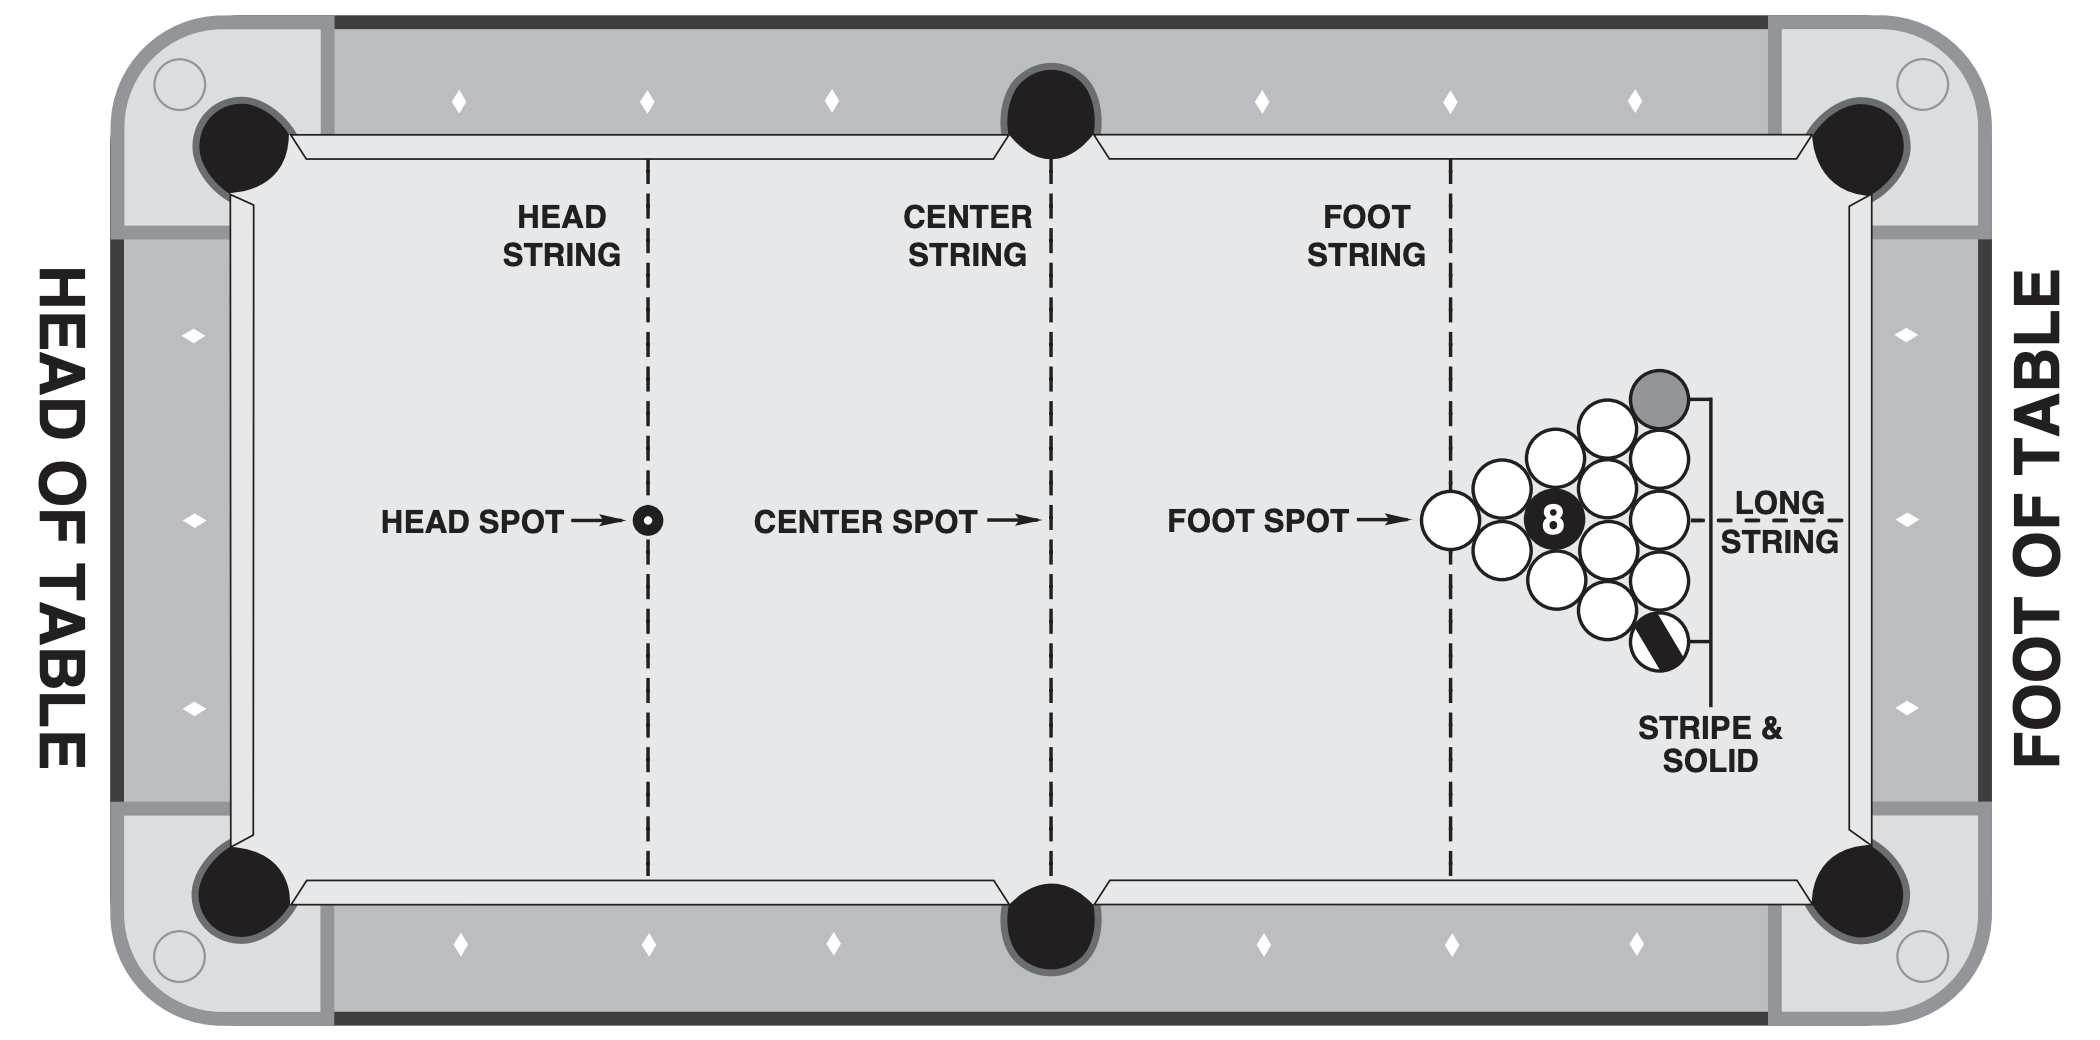
\includegraphics[width=0.75\textwidth]{PoolSplit.png}
\end{figure}

\noindent \emph{I. INIZIO ('BREAK')}

La bilia bianca è posizionata nella posizione di 'head spot'.

Le bilie colorate sono raggruppate in un triangolo equilatero (pieno) di lato pari a 5 bilie.

La bilia 1 è posizionata nella posizione di 'foot spot' e costituisce il vertice del triangolo in direzione della bilia bianca.

Nelle posizioni corrispondenti ai due vertici rimanenti sono posizionate una bilia piena e una bilia spezzata\footnote{Le bilie che si trovano in corrispondenza dei due vertici inferiori del triangolo sono quelle con maggiore probabilità di essere imbucate al momento della spaccata. Per rendere uguale la probabilità che una bilia piena o una bilia spezzata sia imbucata durante la spaccata, si inseriscono in tali posizioni una bilia piena e una bilia spezzata.}.

Le posizioni rimanenti del triangolo, eccetto quella centrale dove è inserita la bilia nera\footnote{La bilia al centro del triangolo è quella con minore probabilità di essere imbucata al momento della spaccata. Per questo, ci si posiziona la bilia nera.}, sono riempite con le bilie rimanenti in modo casuale.

\vspace{9mm}
\noindent \emph{II. ASSEGNAZIONE}

A seguito del break, se è stata imbucata almeno una bilia colorata (che non sia la nera), il giocatore che ha spaccato rimane al tavolo.
Altrimenti, passa al tavolo l'altro giocatore.

A partire dal secondo tiro, al giocatore che per primo imbuca una bilia piena o spezzata, viene assegnata la categoria corrispondente.
All'altro giocatore viene assegnata l'altra.\footnote{Una qualsiasi bilia imbucata nel break non assegna la categoria corrispondente.}

Da questo momento, il giocatore ha l'obbligo di colpire per prima una delle proprie bilie e ha diritto a rimanere al tavolo finché continuerà ad imbucarle in modo regolare.

\vspace{9mm}
\noindent \emph{III. FALLI}

Si verificano situazioni di fallo nei seguenti casi:
\begin{itemize}[noitemsep]
    \item[--]la bilia bianca viene imbucata;
    \item[--] la bilia bianca non colpisce nessuna bilia;
    \item[--] viene colpita una bilia dell'avversario;
    \item[--] viene colpita la bilia nera quando ancora non sono state imbucate tutte le proprie bilie.
\end{itemize}

\pagebreak
In quattro casi l'avversario vince direttamente la partita:
\begin{itemize}[noitemsep]
    \item[--] quando viene imbucata la bilia nera ma ancora non sono state imbucate tutte le proprie bilie;
    \item[--] quando viene imbucata la bilia nera in una buca diversa da quella dichiarata;
    \item[--] quando la bilia bianca viene imbucata dopo la bilia nera.
\end{itemize}

Se un giocatore commette un fallo, il giocatore avversario (passato al tavolo) ha il vantaggio di poter posizionare la bilia bianca in una qualsiasi posizione del tavolo.

\vspace{9mm}
\noindent \emph{IV. FINE}

Una volta che un giocatore ha imbucato tutte e sette le proprie bilie può colpire e imbucare la bilia nera , dichiarando la buca.
Il giocatore che imbuca la bilia nera vince.

\section{L'applicazione JPool}\label{se:JPool} % SECTION 1.2
L'applicazione JPool implementa il gioco del biliardo attraverso una grafica bidimensionale, che rappresenta il piano del tavolo visto dall'alto.

\vspace{3mm}

La simulazione del colpo, effettuato tramite la stecca, è realizzata con una stecca grafica la cui punta è posizionata esattamente dove si trova la bilia bianca.
Mantenendo fissa la punta, è possibile ruotare radialmente la stecca per indirizzare il colpo.
Inoltre, l'utente può regolare la potenza del tiro e, graficamente, viene mostrato un adeguato caricamento della stecca.

\vspace{3mm}

Un giocatore può indirizzare la bilia bianca tramite il puntatore del mouse.
Il videogioco mostra la linea che congiunge la bilia bianca e la posizione desiderata; e in tale posizione genera la 'ghost ball'.
La 'ghost ball' rappresenta graficamente la posizione della bilia bianca al momento della collisione con la palla che si intende colpire.

\vspace{3mm}

Inoltre, nella modalità \emph{Facile} sono mostrate le traiettorie in uscita della bilia che si intende colpire e della bilia bianca a seguito di collisione.
Al variare della posizione del puntatore del mouse in corrispondenza dei punti circostanti la bilia che si intende colpire, variano le traiettorie in uscita. 

\vspace{3mm}

Al fine di rendere l'esperienza di gioco più dinamica, l'applicazione limita il tempo a disposizione per effettuare un colpo a 30 secondi.
La scadenza del tempo a disposizione prima di aver effettuato il tiro comporta il fallo.

\chapter{Specifica dei Requisiti}\label{ch:Specifications} % CHAPTER 2
L'applicazione JPool dovrà soddisfare i seguenti requisiti:
\begin{enumerate}
    \item Rispetto delle leggi fisiche e matematiche coinvolte: la dinamica del gioco deve tenere conto delle dinamiche reali (Legge degli Urti, Forza d'Attrito, Legge di Riflessione), ma allo stesso tempo deve realizzarne un modello approssimato per garantire un adeguato livello di difficoltà;
    \item Rispetto delle regole del gioco 'Palla 8' sopra elencate;
    \item Fluidità del gioco: l'animazione delle bilie in movimento deve essere fedele alle dinamiche reali, producendo un movimento lineare e privo di lag;
    \item Effetto tridimensionale: la GUI deve fornire una parvenza reale del gioco mediante giochi di ombre e altre eventuali tecniche;
    \item Menu di avvio
    \begin{itemize}
        \item[$\rightarrow$] \emph{Play}: consente di avviare una partita
        \begin{itemize}
        	\item[$\rightarrow$] \emph{Settings}: permette di modificare la grafica, le impostazioni audio e il livello di difficoltà relativamente alla partita avviata
        \end{itemize}
        \item[$\rightarrow$] \emph{How to Play}: fornisce una descrizione dettagliata dei comandi necessari per giocare
        \item[$\rightarrow$] \emph{Exit}: termina ed esce dal gioco
    \end{itemize}
    \item Personalizzazione grafica: possibilità di personalizzare il tavolo e la stecca di gioco;
    \item Presenza di audio: urto tra bilie, bilia imbucata, cambio turno, fallo commesso, ticchettio tempo a disposizione, vittoria;
   	\pagebreak
    \item Diversi livelli di difficoltà
    \begin{itemize}
        \item[$\rightarrow$] \emph{Facile}: sono mostrate le anteprime delle traiettorie in uscita (Figura \ref{fig:easyMode})
        \item[$\rightarrow$] \emph{Difficile}: non sono mostrate le anteprime delle traiettorie in uscita (Figura \ref{fig:hardMode})
    \end{itemize}
\end{enumerate}

\begin{figure}[h]
\centering
 \begin{subfigure}{.35\textwidth}
    \centering
    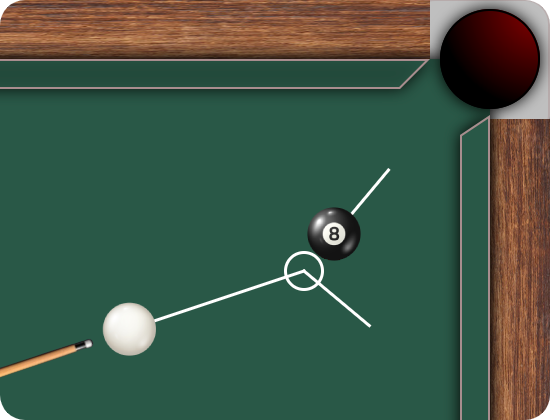
\includegraphics[width=.95\linewidth]{Mode1.png}
    \caption{Modalità Facile.}
    \label{fig:easyMode}
 \end{subfigure}
 \begin{subfigure}{.35\textwidth}
    \centering
    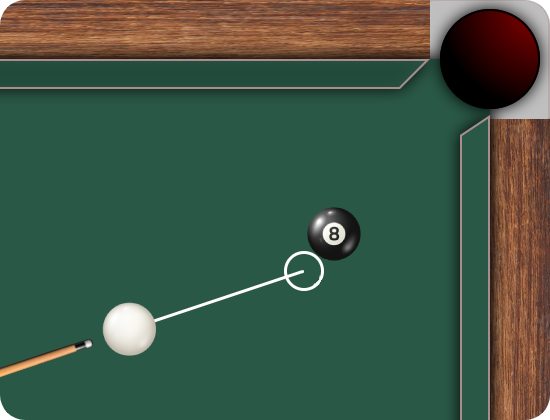
\includegraphics[width=.95\linewidth]{Mode2.png}
    \caption{Modalità Difficile.}
    \label{fig:hardMode}
 \end{subfigure}
\end{figure}

\chapter{Progetto}\label{ch:Project} % CHAPTER 3
Si descrive ora la struttura dell'applicazione realizzata, illustrandone prima l'architettura software e scendendo poi nel dettaglio dei blocchi funzionali che la compongono.

\section{Architettura del Software}\label{se:Software Architecture} % SECTION 3.1

Per semplificare lo sviluppo dell'applicazione si è scelto di seguire un'architettura monolitica: tutte le componenti e tutte le funzionalità del software appartengono ad un unico blocco (monolite).

Nonostante ciò, le classi e le risorse che compongono l'applicazione sono state suddivise in pacchetti; ognuno dei quali ha un preciso ruolo.

\vspace{3mm}

Il pacchetto \texttt{game.entities} comprende le entità direttamente coinvolte nello svolgimento del gioco: i giocatori, le bilie e la loro posizione e velocità nel piano di gioco.

\vspace{3mm}

Il pacchetto \texttt{game.logic} comprende le classi che codificano le regole del gioco e che gestiscono i cambiamenti di scena.
Le classi di tipo 'FXML controller' sono collegate alle rispettive scene di gioco (FXML) e permettono di associare metodi alle componenti grafiche presenti in esse.

\vspace{3mm}

Il pacchetto \texttt{game.resources} non solo contiene le immagini e i suoni presenti nell'applicazione, ma contiene anche i file di definizione e di personalizzazione dell'interfaccia grafica presentata all'utente.
In particolare, il pacchetto \texttt{game.resources.gui.def} contiene i file FXML che definiscono le componenti e le loro proprietà grafiche statiche presenti nelle scene dell'applicazione; mentre il pacchetto \texttt{game.resources.gui.style} contiene i file CSS che permettono di aggiungere proprietà grafiche in modo dinamico.

\vspace{3mm}

Il pacchetto \texttt{game.utils} comprende le classi rimanenti, di varia utilità nello sviluppo del software.


\section{Descrizione dei Pacchetti}\label{se:Packages Description} % SECTION 3.2

\subsection{Entities}\label{se:Entities} % SECTION 3.2.1

\subsubsection*{VECTOR}
La classe \texttt{Vector.java} rappresenta un vettore bidimensionale uscente dall'origine del Pane.
I metodi della classe implementano le operazioni vettoriali di:
\begin{itemize}
	\item [--] somma (\texttt{add(Vector v)})
	\item [--] differenza (\texttt{sub(Vector v)})
	\item [--] moltiplicazione scalare (\texttt{multiply(double k)})
	\item [--] prodotto scalare (\texttt{scalar(Vector v)})
	\item [--] normalizzazione (\texttt{normalize()})
	\item [--] vettori perpendicolari (\texttt{perpendicularLeft()}, \texttt{perpendicularRight()}) 
\end{itemize}
Un vettore può anche invocare il metodo \texttt{determinant(Vector a, Vector b)}, che restituisce il determinante della seguente matrice:
\[
\begin{pmatrix}
\texttt{this.x - a.getX()} & \texttt{b.getX() - a.getX()}\\
\texttt{this.y - a.getY()} & \texttt{b.getY() - a.getY()}
\end{pmatrix}
\]

\vspace{3mm}

\subsubsection*{BALL}
La classe \texttt{Ball.java} implementa il modello fisico (tridimensionale) di una bilia.
Dato che tutte le bilie in gioco hanno stessa dimensione, i dati da specificare per la creazione di una bilia sono la sua posizione nel piano (Pane) e il suo numero.

\vspace{3mm}

Il metodo \texttt{drawBall()} restituisce un nodo di tipo Sphere caratterizzato da un determinato raggio e da effetti grafici quali:
\begin{itemize}
	\item [--] \texttt{PhongMaterial}\cite{PhongMaterial}, che, data una componente diffusa (grafica della superficie esterna della bilia) e una componente speculare (colore bianco), realizza la riflessione della luce.
	\item [--] \texttt{DropShadow}\cite{DropShadow}, che realizza l'ombra specificandone la profondità radiale e lo spostamento lungo gli assi x e y.
\end{itemize}

Il metodo \texttt{triangle()} crea e dispone le 16 bilie in gioco per la spaccata iniziale come da regolamento.

\vspace{3mm}

Il metodo \texttt{ballAnimation(int ballNum)}, collegato alla Timeline dell'applicazione, realizza l'animazione di una bilia.
Nel dettaglio, chiama il metodo \texttt{spin()} per far ruotare la bilia su se stessa rispetto gli assi x e y, il metodo \texttt{bankCollision()} per modificare la velocità della bilia a seguito di un urto con una sponda e il metodo \texttt{tableFriction()} per modificare la velocità della bilia a causa della forza d'attrito del tavolo di gioco.
Inoltre, grazie al controllo del metodo \texttt{collides(Ball b)}, se la bilia in input è in collisione con una qualsiasi bilia in gioco, il metodo \texttt{ballCollision()} modifica la velocità di entrambe le bilie in collisione.

\vspace{3mm}

Il metodo \texttt{checkPocket(int ballNum)} collegato alla Timeline dell'applicazione, controlla se la bilia in input è "contenuta" in una delle buche del tavolo di gioco e, in caso positivo, chiama il metodo \texttt{pocketed(int ballNum)} che si occupa di eliminare la bilia dal tavolo di gioco e di inserirla nel rack laterale.

\subsubsection*{PLAYER}
La classe \texttt{Player.java} rappresenta un giocatore.
Per la creazione di un giocatore è sufficiente fornire un nickname.
I restanti attributi del giocatore sono necessari per l'implementazione delle regole del gioco; infatti ci permettono di conoscere (in ogni momento della partita) quale dei due giocatori deve colpire, la categoria di bilie assegnata a ciascun giocatore e, a fine partita, quale dei due giocatori ha vinto.

\subsection{Logic}\label{se:Logic} % SECTION 3.2.2

\subsubsection*{MENU CONTROLLER}
Il controller \texttt{MenuController.java} è associato alla schermata \texttt{Menu.fxml} e fornisce tre metodi da eseguire alla pressione di ciascuno dei tre pulsanti presenti nella scena.
Il pulsante START GAME, gestito dal metodo \texttt{handleStartGameButton()}, carica la scena che permette di personalizzare una partita.
Il pulsante HOW TO PLAY, gestito dal metodo \texttt{handleHTPButton()}, carica la scena esplicativa delle modalità di gioco.
Il pulsante EXIT, gestito dal metodo \texttt{handleExitButton()}, chiude la finestra (Stage) e termina l'applicazione.

\subsubsection*{SETTINGS CONTROLLER}
Il controller \texttt{SettingsController.java} è associato alla schermata FXML delle impostazioni di gioco e gestisce gli input dell'utente relativamente alla personalizzazione di una partita.
Per la scelta del tavolo, della stecca e della difficoltà di gioco si è scelto di utilizzare la componente grafica Pagination.
Quest'ultima permette di definire una sottoscena contenente diverse pagine indicizzate.
Ogni pagina può contenere diversi componenti ed è selezionabile dall'utente tramite appositi pulsanti grafici.
Le tre paginazioni \texttt{tableMenu}, \texttt{cueMenu}, \texttt{modeMenu} sono definite nel metodo \texttt{initialize()} sfruttando il metodo \texttt{setPageFactory(...)}, che permette di specificare un Node da inserire in ogni pagina.
Una proprietà fondamentale di un oggetto Pagination è quella di poter chiamare in ogni momento il metodo \texttt{getCurrentPageIndex()} per conoscere la pagina selezionata dall'utente e, di conseguenza, selezionare la grafica desiderata.

\subsubsection*{GAME CONTROLLER}
Il controller \texttt{GameController.java} è associato alla schermata \texttt{Game.fxml} e, oltre a dirigere la partita nel tempo, contiene metodi che implementano l'esecuzione di un tiro.

\vspace{3mm}

Il metodo \texttt{initialize()} si occupa di impostare correttamente la grafica e la logica (variabili di controllo) all'inizio di ogni partita.
Si occupa principalmente di:
\begin{itemize}
	\item [--] stabilire quale dei due giocatori deve iniziare, comunicando con il controller delle impostazioni di gioco;
	\item [--] caricare la stecca di gioco selezionata, comunicando con il controller delle impostazioni di gioco;
	\item [--] configurare le bilie per la spaccata iniziale, invocando il metodo \texttt{triangle()} della classe \texttt{Ball.java}.
\end{itemize}

\vspace{3mm}

La grafica dell'esecuzione di un tiro è implementata tramite le seguenti componenti della scena FXML:
\begin{itemize}
	\item [--] \texttt{Line guidelineToBall}, cioè la linea che congiunge la bilia bianca e la bilia che si vuole colpire;
	\item [--] \texttt{Circle ghostBall}, cioè la previsione della bilia bianca al momento dell'urto;
	\item [--] \texttt{Line guidelineFromBall}, cioè la linea che mostra la traiettoria della bilia colpita dopo la collisione;
	\item [--] \texttt{Line guidelineFromCue}, cioè la linea che mostra la traiettoria della bilia bianca dopo la collisone.
\end{itemize}
I metodi che permettono all'utente di visualizzare la grafica di un tiro e poi di effettuare un tiro sono i seguenti.

Il metodo \texttt{guidedTrajectory(MouseEvent event)} mostra all'utente, al variare della posizione del puntatore del mouse, la grafica necessaria per poter effettuare un tiro.
Questo metodo svolge principalmente due compiti:
\begin{itemize}
	\item [--] aggiorna la grafics mostrando all'utente la \texttt{guidelineToBall}, la \texttt{ghostBall}, la \texttt{guidelineFromBall} e la \texttt{guidelineFromCue};
	\item [--] aggiorna la grafica ruotando la stecca intorno alla bilia bianca adeguatamente rispetto alla direzione del colpo (posizione del mouse).
\end{itemize}

Il metodo \texttt{fixTrajectory(MouseEvent event)} è associato alla scena FXML tramite l'azione di rilascio del mouse e memorizza le componenti x e y di rilascio del mouse in due apposite variabili d'istanza.

Il metodo \texttt{cueLoading()} permette di caricare il colpo, regolandone la potenza.
Questo metodo si occupa di aggiornare la grafica mostrando all'utente la potenza del tiro che si vuole effettuare in base a quanto ha trascinato l'apposito slider verso il basso.
Allo stesso tempo, fissata la posizione radiale della stecca intorno alla bilia bianca, la si trasla adeguatamente rispetto alla potenza scelta in direzione opposta rispetto a quella del tiro che si vuole effettuare; emulando il reale caricamento di un colpo.

Il metodo \texttt{cueShot()} è associato alla scena FXML tramite l'azione di rilascio dello slider e si occupa di far partire il colpo.
Nello specifico, imposta il vettore velocità della bilia bianca in direzione della bilia che si vuole colpire (coordinate x e y mouse released) e lo moltiplica scalarmente per la velocità della bilia bianca impostata tramite lo slider di potenza.

\begin{lstlisting}[language = Java , frame = trBL, escapeinside={(*@}{@*)}]

	cueBallVelocity = powerSlider.getValue();
	
    double angle = Math.atan2(yMouseReleased - ball[0].getPosition().getY(), xMouseReleased - ball[0].getPosition().getX());
    
	setCueVelocity(cueBallVelocity * Math.cos(angle), cueBallVelocity * Math.sin(angle));
	
\end{lstlisting}

La funzione \texttt{Math.atan2(y, x)} permette di determinare l'angolo formato da un vettore \texttt{(x, y)} con l'asse x di un piano con polo nell'origine.
Per determinare la direzione e il verso della bilia bianca, si vuole determinare l'angolo formato dal vettore \texttt{(xMouseReleased, yMouseReleased)} con l'asse delle ascisse di un piano cono polo nel centro della bilia bianca \texttt{(ball[0].getPosition().getX(), ball[0].getPosition().getY()}.

Noto l'angolo, si scompone la velocità della bilia bianca lungo x e y sfruttando le funzioni trigonometriche \texttt{Math.cos()} e \texttt{Math.sin()} e la si moltiplica scalarmente per la velocità impostata dallo slider.

\vspace{3mm}

Dato che una partita si gioca nel tempo, è necessario definire un "asse temporale" a cui siano associati i metodi necessari alla creazione delle animazioni e allo svolgimento della partita.
A tal proposito si è scelto di utilizzare la classe \texttt{Timeline}.
Contestualmente al caricamento del file \texttt{Game.fxml} nel metodo \texttt{initialize()} viene creata la timeline e viene chiamato il metodo \texttt{startGame()}.
Quest'ultimo imposta il periodo di aggiornamento di ogni frame a 0.015 secondi \footnote{La scelta del frame rate è stata fatta consultando altri progetti di videogiochi e facendo diversi tentativi.} e imposta la lunghezza della timeline come indefinita; in modo che la partita possa continuare fino a che non si determini un vincitore.
Quindi, avvia la timeline (inizia l'animazione) e ad ogni aggiornamento di frame viene invocato il metodo \texttt{update()}.

\vspace{3mm}

Il metodo \texttt{update()} svolge diversi compiti, ma principalmente:
\begin{itemize}
	\item [--] invoca i metodi \texttt{ballAnimation(int ballNum)} e \texttt{checkPocket(int ballNum)} per tutte le bilie in gioco, in modo da aggiornare la posizione delle bilie e, se si trovano in una delle buche del tavolo, mandarle in buca;
	\item [--] controlla se tutte le bilie in gioco sono ferme e, in tal caso, aggiorna la logica e la grafica del gioco sulla base di ciò che si è verificato al turno precedente (bilie imbucate, falli).
\end{itemize}

\subsubsection*{RULES}
La classe \texttt{Rules.java} contiene metodi (collegati alla Timeline) che permettono di controllare l'andamento della partita e il rispetto delle regole di gioco (falli).

\vspace{3mm}

Il metodo \texttt{checkFoul()} svolge diversi compiti necessari al corretto svolgimento di una partita come da regolamento ed è infatti richiamato dal metodo \texttt{update()} alla fine di ogni turno.
Si occupa principalmente di gestire i cambi di turno, di gestire l'assegnazione delle bilie e di controllare e segnalare i falli.

\vspace{3mm}

Il metodo \texttt{checkPotted()} controlla se tutte le bilie di una categoria assegnata ad un giocatore sono state imbucate e in tal caso assegna al giocatore tale proprietà.

\subsubsection*{BOARD}
La classe \texttt{Board.java} contiene metodi (collegati alla Timeline) che mostrano all'utente informazioni utili al rispetto delle regole di gioco.
Nello specifico, aggiorna i seguenti Label presenti nella scena di gioco: \texttt{scoreboardLabel}, \texttt{centralboardLabel} e \texttt{foulboardLabel}.
Il primo specifica in ogni momento quale dei due giocatori è al tavolo, il secondo notifica l'assegnazione delle bilie ai giocatori, la vittoria di un giocatore ed è anche utilizzato quando si vuole terminare la partita; il terzo notifica i falli rilevati e ne specifica il tipo.

\subsection{Resources}\label{se:Resources} % SECTION 3.2.3

Oltre alle immagini e ai suoni, questa sezione contiene i file di definizione (FXML) e personalizzazione (CSS) della GUI.

\subsubsection*{FXML}
Ad ogni schermata di gioco corrisponde un file FXML che ne definisce la struttura grafica e che contiene i metodi da eseguire in risposta agli input dell'utente (eventi).
Per la realizzazione della parte statica delle schermate di gioco si è utilizzato il software SceneBuilder, fornito dal framework JavaFX. \cite{JavaFX}

\subsubsection*{CSS}
Contestualmente al caricamento di ogni schermata tramite FXMLLoader, viene aggiunta la 'stylesheet' \texttt{standard.css}.
Quest'ultima contiene una serie di proprietà grafiche, relative ai vari componenti delle schermate, che caratterizzano lo stile dell'applicazione.
Le proprietà grafiche sono specificate principalmente su classi di componenti, piuttosto che su un singolo componente; perché si vuole creare uno stile grafico preciso e univoco per ogni componente dell'applicazione.
Ad esempio, la classe dei pulsanti dell'applicazione fa riferimento allo stile mostrato in Figura \ref{fig:ButtonStyle}.

\begin{figure}
    \centering
    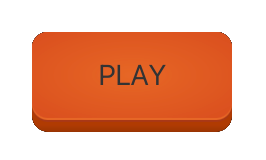
\includegraphics[width=0.25\textwidth]{ButtonStyle.png}
    \caption{Stile grafico dei pulsanti di JPool.}
    \label{fig:ButtonStyle}
\end{figure}

Sono inoltre presenti quattro file CSS per la personalizzazione grafica del tavolo di gioco.
In base alla scelta dell'utente nella schermata di impostazioni di gioco, viene caricata dinamicamente una precisa configurazione che modifica il legno esterno del tavolo e il colore del piano di gioco e delle sponde.
Le componenti da modificare sono incluse in una precisa 'CSS style class' (table, bank) in modo da poter essere referenziate nella 'CSS stylesheet' caricata (\texttt{table1,2,3,4.css}).

\subsection{Utils}\label{se:Utils} % SECTION 3.2.4
La classe \texttt{Constants.java} contiene costanti utili allo sviluppo del gioco.

Ad esempio, nella sezione \texttt{//SPLIT} sono tabulate tutte le coordinate x e y necessarie al raggruppamento delle bilie nel triangolo del break.

\vspace{3mm}

La classe \texttt{Sounds.java} permette di riprodurre effetti sonori.

\section{Problemi Riscontrati}\label{se:Issues} % SECTION 3.3
Durante lo sviluppo del videogioco sono stati riscontrati problemi di diversa natura.

\vspace{3mm}

Problemi di natura tecnica, cioè riguardanti la sintassi e la semantica della tecnologia utilizzata (JavaFX), sono stati risolti consultando la documentazione ufficiale (JavaFX API) oppure consultando domande (e relative risposte) inerenti nel sito stackoverflow.com.

\vspace{3mm}

Problemi di natura logica, cioè relativi al corretto funzionamento del software e all'assoluzione delle specifiche, sono stati trattati caso per caso con diversi metodi.

\subsubsection*{TRAIETTORIA BILIA BIANCA}
Il calcolo della traiettoria della bilia bianca dopo un'ipotetica collisione con un'altra bilia ha richiesto particolare attenzione.
Infatti, l'utente sposta la ghost ball intorno a una bilia che vuole colpire per visualizzare le traiettorie post collisone e, solo dopo aver trovato la direzione desiderata, carica e rilascia il colpo; assegnando una certa velocità alla bilia bianca.
Il problema è che, quando l'utente sta decidendo la direzione del colpo, non esiste un vettore velocità della bilia bianca (da applicare al centro della ghost ball) che ci permetta di calcolare le velocità finali come nel metodo \texttt{ballCollision(int ballNum)}.

Il vettore traiettoria delle bilia che si intende colpire (\texttt{ballFinalVelocity}) è stato calcolato assumendo una velocità scalare della bilia bianca (\texttt{cueBallVeloctiy}) pari a 50.

Per il vettore traiettoria della bilia bianca (\texttt{cueFinalVelocity}), si è deciso di calcolarlo come uno dei due vettori perpendicolari al vettore \texttt{ballFinalVelocity}. In effetti, in una collisione bidimensionale tra due bilie è sempre vero che le bilie seguono direzioni tra di loro ortogonali. Resta solo da stabilire adeguatamente il verso del vettore ortogonale, infatti può essere tanto in una direzione quanto nell'altra.

\vspace{3mm}

La soluzione a quest'ultimo problema è stata trovata notando che: ruotando la ghost ball attorno alla bilia da colpire, questa dovrà andare in un verso se il suo centro si trova alla sinistra della linea \texttt{guidelineToBall} (che unisce la bilia bianca e la bilia da colpire), nel verso opposto altrimenti.
La condizione che, dati tre punti, permette di determinare se un punto si trova a sinistra o a destra di una retta (individuata dagli altri due) è fornita dal segno del determinante della matrice:

\[
\begin{pmatrix}
\texttt{x - x1} & \texttt{x2 - x1}\\
\texttt{y - y1} & \texttt{y2 - y1}
\end{pmatrix}
\]

dove $P = (x, y)$ è il punto da verificare e $P_1 = (x_1, y_1), P_2 = (x_2, y_2)$ sono i punti che individuano la retta.\cite{PointSideLineMath}\cite{PointSideLineCode}

\vspace{3mm}

Il metodo \texttt{determinant(Vector a, Vector b)}, trattato nella sezione \ref{se:Entities}, è stato realizzato a tale scopo.
Il punto (vettore) che invoca il metodo è il punto che si vuole verificare (centro ghostball), mentre i due punti in input individuano la retta (centro bilia bianca, centro bilia da colpire).

\vspace{3mm}

Se il determinante è positivo, allora il punto si trova a sinistra della retta e quindi il vettore \texttt{cueFinalVelocity} è il perpendicolare sinistro di \texttt{ballFinalVelocity}.
Se il determinante è negativo, allora il punto si trova a destra della retta e quindi il vettore \texttt{cueFinalVelocity} è il perpendicolare destro di \texttt{ballFinalVelocity}.
Se il determinante è nullo, allora il punto giace sulla retta e quindi il vettore \texttt{cueFinalVelocity} ha stessa direzione e verso di \texttt{ballFinalVelocity}; per questo si imposta come nullo.

\subsubsection*{SOVRAPPOSIZIONE SUONI}
L'applicazione prevede l'esecuzione di effetti sonori in diverse circostanze. Una di queste è l'urto tra due bilie.

\vspace{3mm}

Al momento della spaccata, le bilie sono raggruppate in modo compatto in un triangolo. Quando uno dei due giocatori spacca, colpendo (in generale) la bilia sulla punta del triangolo, si verificano molti urti tra bilie.

Dato che ogni urto riproduce l'effetto sonoro di collisione, si sovrappongono in un breve intervallo temporale tanti suoni.
Testando l'applicazione, si è notato che, talvolta, questa fitta riproduzione e sovrapposizione di suoni manda in blocco il software.

\vspace{3mm}

Si è risolto il problema disattivando l'effetto sonoro di collisone per il primo tiro avviando un suono di spaccata iniziale.


\chapter{Appendice}\label{ch:Appendix} % CHAPTER 4
In questo capitolo si entra nel dettaglio di alcuni metodi di particolare interesse nello sviluppo dell'applicazione, scendendo nel dettaglio dei concetti matematici, fisici e logici che li rendono operativi.

\subsubsection*{URTO BILIA-BILIA}

\begin{lstlisting}[language = Java , frame = trBL, escapeinside={(*@}{@*)}]
public void ballCollision(Ball b) {

        Vector n1 = position.sub(b.position);
        n1.normalize(); // un1
        double v1n = velocity.scalar(n1);
        n1.multiply(v1n); // v1n (vector)
        Vector v1t = velocity.sub(n1);

        Vector n2 = b.position.sub(position);
        n2.normalize(); // un2
        double v2n = b.velocity.scalar(n2);
        n2.multiply(v2n); // v2n (vector)
        Vector v2t = b.velocity.sub(n2);
        
        velocity = v1t.add(n2);
        b.velocity = v2t.add(n1);
        
}
\end{lstlisting}

\pagebreak

La collisione tra due bilie\cite{2DCollision} è un urto di tipo elastico. Questo significa che nella collisione si conservano sia la quantità di moto che l'energia cinetica.

Le equazioni di conservazione in uno spazio monodimensionale sono le seguenti:
\[m_1v_1 + m_2v_2 = m_1v_1' + m_2v_2'\]
\[\frac{1}{2}m_1v_1^2 + \frac{1}{2}m_2v_2^2 = \frac{1}{2}m_1v_1'^2 + \frac{1}{2}m_2v_2'^2\]

Dalle quali si ricavano le velocità finali:
\[v_1' = \frac{v_1(m_1 - m_2) + 2m_2v_2}{m_1 + m_2} \qquad v_2' = \frac{v_2(m_2 - m_1) + 2m_1v_1}{m_1 + m_2}\]

Per il contesto di interesse è possibile fare l'ipotesi $m_1 = m_2 = 1$, visto che tutte le bilie hanno stessa massa, quindi le velocità finali diventano:
\[v_1' = v_2 \qquad v_2' = v_1\]

\begin{wrapfigure}{r}{0.5\textwidth}
  \begin{center}
  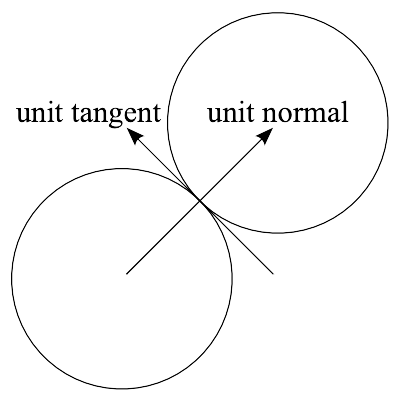
\includegraphics[width=0.4\textwidth]{2DCollision.png}
  \end{center}

\end{wrapfigure}

In una collisione bidimensionale si proiettano le velocità lungo due direzioni: una direzione perpendicolare alla superficie dell'impatto (normale), una direzione parallela alla superficie dell'impatto (tangente).
Questo significa che ogni vettore velocità sarà caratterizzato da una componente normale e da una tangenziale.

La componente tangenziale del vettore velocità rimane costante nella collisione perché non c'è alcuna forza in tale direzione.

La componente normale, invece, cambia seguendo la legge unidimensionale trattata sopra.

\vspace{3mm}

Il metodo, sfruttando le operazioni definite nella classe \texttt{Vector.java}, calcola le velocità normali $v_1^n, v_2^n$ e le velocità tangenziali $v_1^t, v_2^t$\footnote{Le velocità normali $v_1^n, v_2^n$ sono di fatto i vettori $n_1, n_2$, visto che i metodi utilizzati non restituiscono un vettore; ma modificano l'invocante.}; per poi determinare le medesime dopo la collisione e, quindi, calcolare le velocità finali.

In particolare, per ogni bilia:
\begin{enumerate}
	\item si determina la direzione normale sottraendo i vettori 
	\item si normalizza il vettore, ottenendo l'unità normale
	\item si proietta (prodotto scalare) la velocità della bilia lungo l'unità normale, ottenendo il valore scalare della velocità della bilia lungo la componente normale
	\item si moltiplica (scalarmente) l'unità normale per il risultato ottenuto al punto 3, ottenendo $v_{1,2}^n$
	\item si determina la velocità tangenziale ($v_{1,2}^t$) sottraendo alla velocità la velocità normale
\end{enumerate}

Infine, il metodo determina i vettori finali \texttt{velocity} (velocità bilia invocante) e \texttt{b.velocity} (velocità bilia in input) sommando la velocità normale e la velocità tangenziale della bilia dopo la collisione.
I vettori $v_1^n, v_2^n$ (nel metodo $n_1, n_2$) sono scambiati in accordo con la legge della dinamica monodimensionale; mentre i vettori $v_1^t, v_2^t$ si conservano nella collisione.

\pagebreak
\subsubsection*{URTO BILIA-SPONDA} 

\begin{lstlisting}[language = Java , frame = trBL, escapeinside={(*@}{@*)}]
public void bankCollision() {

        double x = position.getX();
        double y = position.getY();
        double r = Constants.BALL_RADIUS;

        // LEFT BANK (A)
        // REGION A1
        if (x - r <= Constants.A_MARGIN && (y >= Constants.A_UP_CORNER_START && y <= Constants.A_UP_CORNER_END)) {
            velocity.setY(-velocity.getSize());
            velocity.setX(0);
        }
        // REGION A2
        else if (x - r <= Constants.A_MARGIN && (y >= Constants.A_UP_CORNER_END && y <= Constants.A_DOWN_CORNER_START)) {
            velocity.setX(Math.abs(velocity.getX()));
        }
        // REGION A3
        else if (x - r <= Constants.A_MARGIN && (y >= Constants.A_DOWN_CORNER_START && y <= Constants.A_DOWN_CORNER_END)) {
            velocity.setY(velocity.getSize());
            velocity.setX(0);
        }
        
        ...
        
}
\end{lstlisting}

\pagebreak

Per gestire l'urto di una bilia con una sponda del tavolo, si è deciso di suddividere ogni sponda in tre zone distinte.
Infatti, dato che ogni sponda è compresa tra due buche del tavolo, è possibile individuare una regione in prossimità di una buca, un'altra in prossimità dell'altra e un'altra ancora compresa tra le due regioni.
Ogni regione in prossimità di una buca è fatta in modo da direzionare la bilia che la colpisce nella direzione della buca.

Per semplificare il problema, si è deciso di far riferimento alle sponde con letterali, come indicato dalla Figura \ref{fig:Banks}.

\begin{figure}[h]
    \centering
    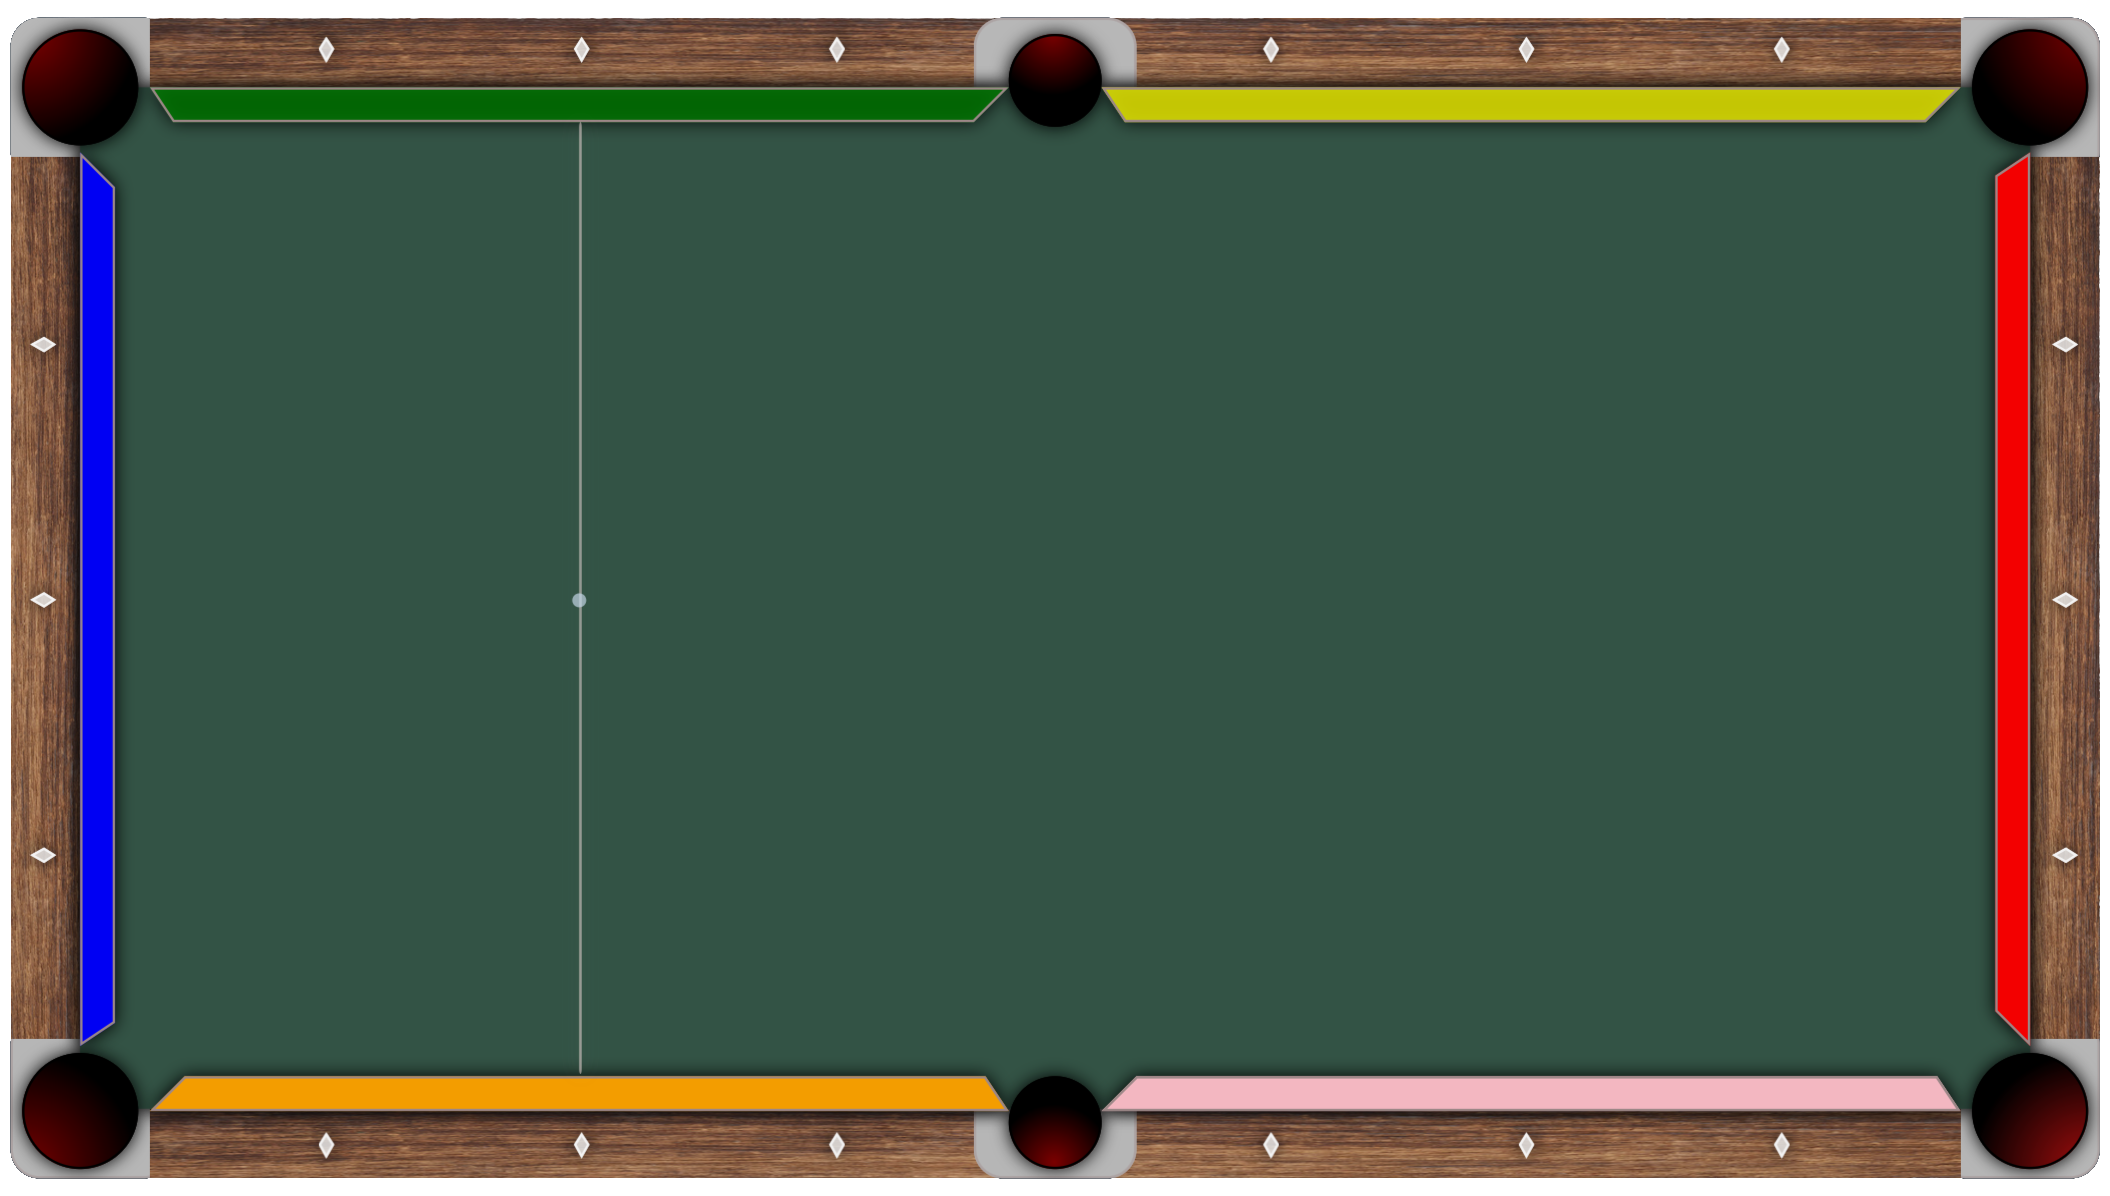
\includegraphics[width=0.4\textwidth]{Banks.png}
    \caption{Blu (A), Rosso (B), Verde (C), Giallo (D), Arancione (E), Rosa (F)}
    \label{fig:Banks}
\end{figure}

Per ogni sponda, le relative regioni sono sempre considerate in ordine crescente rispetto agli assi del piano (Pane). Cioè per le sponde A e B le regioni A1, A2, A3 e B1, B2, B3 sono individuate andando nel verso crescete dell'asse y (dall'alto verso il basso), mentre per le sponde C, D, E, F le regioni C1, C2, C3, D1, D2, D3, E1, E2, E3 e F1, F2, F3 sono individuate andando nel verso crescente dell'asse x (da sinistra verso destra).

\vspace{3mm}

Per semplicità si è riportato solo il codice che controlla l'urto con la sponda A, ma i ragionamenti sono del tutto analoghi per le sponde rimanenti.

Se una bilia urta la regione A2, allora per la Legge di Riflessione \footnote{L'urto di una bilia contro una sponda è assimilabile alla riflessione della luce su uno specchio piano.} si conserva il modulo della velocità.
Inoltre, la componente y conserva il verso della velocità (ad esempio una bilia che urta provenendo dall'altro, cioè con velocità verso il basso, continuerà ad andare verso il basso dopo l'urto).
Lungo x, invece, il verso della velocità sarà sicuramente verso destra, quindi la velocità lungo x viene impostata positiva.

Se una bilia urta la regione A1 o A3, la velocità lungo x sarà sicuramente nulla; visto che la bilia viene indirizzata verso la rispettiva buca.
La velocità lungo y, invece, sarà negativa (verso) e pari al modulo della velocità per la regione A1 (visto che la bilia deve andare verso l'alto) e sarà positiva (verso) e pari al modulo della velocità per la regione A3 (visto che la bilia deve andare verso il basso).

\pagebreak
% BIBLIOGRAPHY
\bibliographystyle{unsrturl}
\bibliography{refs}

\end{document} % DOCUMENT END